\section{设计思想}
% 本程序中用到的所有数据类型的定义,主程序的流程图及各程序模块之间的调用关系
\subsection{逻辑设计}
与二叉树的设计基本上是一致的,实现了泛型的操作,可以支持不同的类型。

\subsubsection{AvlTree}
\begin{lstlisting}[language = c++]
template<typename Comparable>
class AvlTree {
public:
    AvlTree() : root(nullptr) {}
    ~AvlTree() { makeEmpty(root); }
    bool contains(const Comparable &x);
    const Comparable &find(const Comparable &x);
    void insert(const Comparable &x);
    void remove(const Comparable &x);
    void visitTreeCover(const std::function<void(AvlNode *)> &visit);
    void printGraph(std::ostream &out = std::cout);
    void visitTree(const std::function<void(AvlNode *)> &visit);
private:
    AvlNode *root;
};
\end{lstlisting}

\subsubsection{AvlNode}

这是Avl树的结点,用来存储数据。

\begin{lstlisting}[language = c++]
struct AvlNode {
    Comparable element;
    AvlNode *left;
    AvlNode *right;
    int height;
    AvlNode(const Comparable &ele, AvlNode *lt, AvlNode *rt, int h = 0)
        : element(ele), left(lt), right(rt), height(h) {}
    AvlNode(Comparable &&ele, AvlNode *lt, AvlNode *rt, int h = 0)
        : element(std::move(ele)), left(lt), right(rt), height(h) {}
}
\end{lstlisting}

\subsection{整体依赖关系图}

\begin{figure}[H]
    \centering
    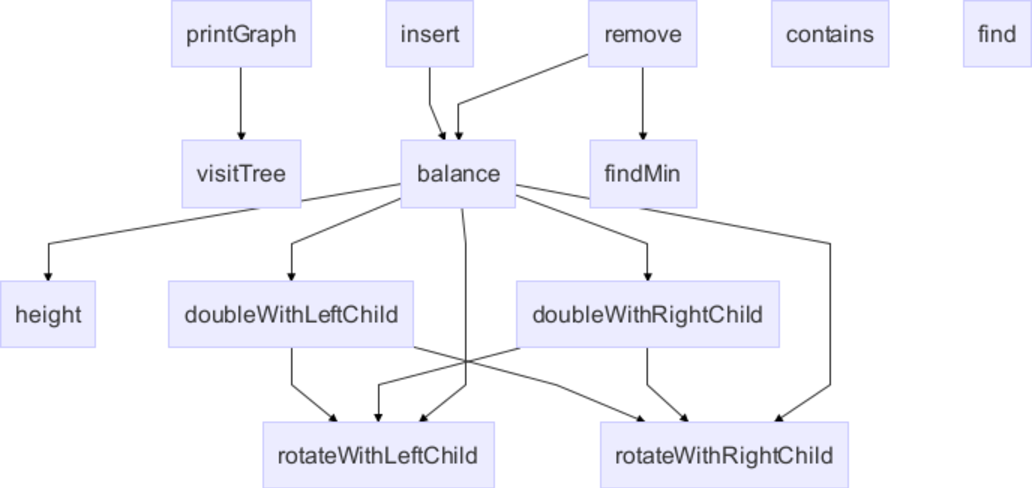
\includegraphics[width=0.7\linewidth]{figures/depends}
    \caption{整体依赖关系图}
    \label{fig:depends}
\end{figure}


\subsection{Main函数流程图}

\begin{figure}[H]
    \centering
    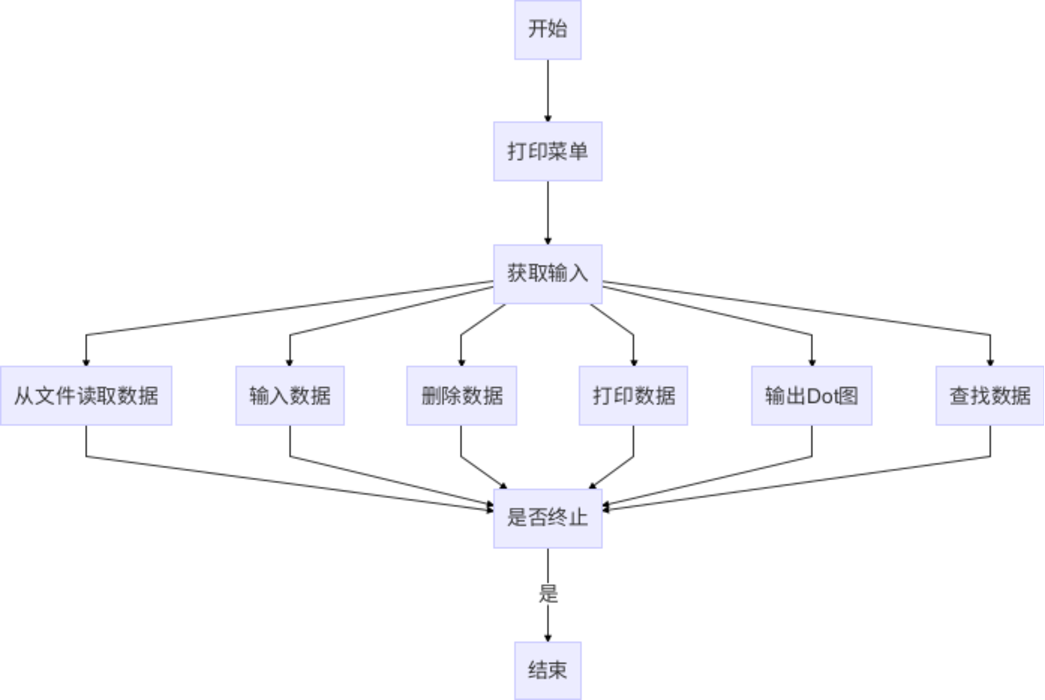
\includegraphics[width=0.7\linewidth]{figures/flowchart}
    \caption{Main函数流程图}
    \label{fig:flowchart}
\end{figure}

